\chapter{Эмпирическое исследование алгоритмов устранения дедлоков}
\label{chap:experiments}

\section{Методология проведения экспериментов}
\label{sec:exp_methodology}

Экспериментальное исследование направлено на оценку устойчивости мезоскопического симулятора трафика и выявление оптимальных параметров буферизации застрявших агентов. Симуляция производилась на дорожном графе города Казани ($N_{\text{edges}} = 160\,689$) с пиковой популяцией $N_{\text{max}} = 70\,000$ автомобилей.

Сравниваются две ключевые конфигурации эмпирического механизма непрерывного таймера (\texttt{conttimer}):
\begin{enumerate}
    \item \textbf{Конфигурация 1 (\texttt{run\_27-07-2026})}: Пороговое время телепортации $T_{\text{teleport}} = 130$ с, непрерывный таймер простоя, продолжительность прогона $172.97$ часов (более 7 суток физического времени симуляции).
    \item \textbf{Конфигурация 2 (\texttt{run\_28-07-2026})}: Пороговое время телепортации $T_{\text{teleport}} = 300$ с, непрерывный таймер простоя, продолжительность прогона $51.71$ час (более 2 суток физического времени симуляции).
\end{enumerate}

В обоих прогонах порог квалификации ребра как «занятого» составлял $J_{\text{thresh}} = 70\%$, а шаг физического такта $\Delta t = 0.1$ с.

\section{Сравнительный анализ метрик симуляции}
\label{sec:runs_comparison}

Сводные результаты экспериментальных прогонов приведены в таблице~\ref{tab:runs_comparison}.

\begin{table}[h!]
\centering
\caption{Сводные показатели эффективности механизмов разблокировки}
\label{tab:runs_comparison}
\begin{tabular}{|l|c|c|}
\hline
\textbf{Показатель / Метрика} & \textbf{Конфигурация 1 (130 с)} & \textbf{Конфигурация 2 (300 с)} \\ \hline
Длительность замера (ч) & $172.97$ & $51.71$ \\ \hline
Всего завершенных поездок & $19\,681\,882$ & $5\,036\,511$ \\ \hline
Средняя популяция на дорогах & $33\,641.9$ авт. & $33\,590.9$ авт. \\ \hline
Пиковая популяция на дорогах & $64\,693$ авт. & $67\,126$ авт. \\ \hline
\textbf{Средний индекс задержки (TTI)} & $\mathbf{1.8881}$ & $\mathbf{2.2515}$ \\ \hline
Максимальный индекс TTI & $5.0323$ & $7.8969$ \\ \hline
Стандартное отклонение TTI ($\sigma$) & $0.2943$ & $0.6450$ \\ \hline
\textbf{Средняя доля застрявших (0 км/ч)} & $\mathbf{23.02\%}$ ($10\,093$ авт.) & $\mathbf{36.24\%}$ ($15\,391$ авт.) \\ \hline
Пиковая доля застрявших (0 км/ч) & $44.67\%$ ($28\,684$ авт.) & $61.13\%$ ($40\,871$ авт.) \\ \hline
\textbf{Средняя доля буфера SUMO} & $\mathbf{5.58\%}$ ($2\,505$ авт.) & $\mathbf{2.90\%}$ ($1\,331$ авт.) \\ \hline
Пиковая доля буфера SUMO & $14.19\%$ ($7\,988$ авт.) & $8.32\%$ ($4\,597$ авт.) \\ \hline
Средняя скорость потока & $41.8$ км/ч & $36.7$ км/ч \\ \hline
Макс. время простоя 1 агента & $130.0$ с & $300.0$ с \\ \hline
Производительность роутера (RPS) & $2\,206.9$ RPS & $2\,556.2$ RPS \\ \hline
\end{tabular}
\end{table}

Для более детального сопоставления характера протекания процессов на установившемся суточном режиме ($0 \dots 24$ ч) произведено срезание последних 24 часов симуляции для обеих конфигураций.

На рисунке~\ref{fig:tti_24h} показано сравнение динамики индекса задержки TTI на протяжении 24-часового цикла.

\begin{figure}[h!]
\centering
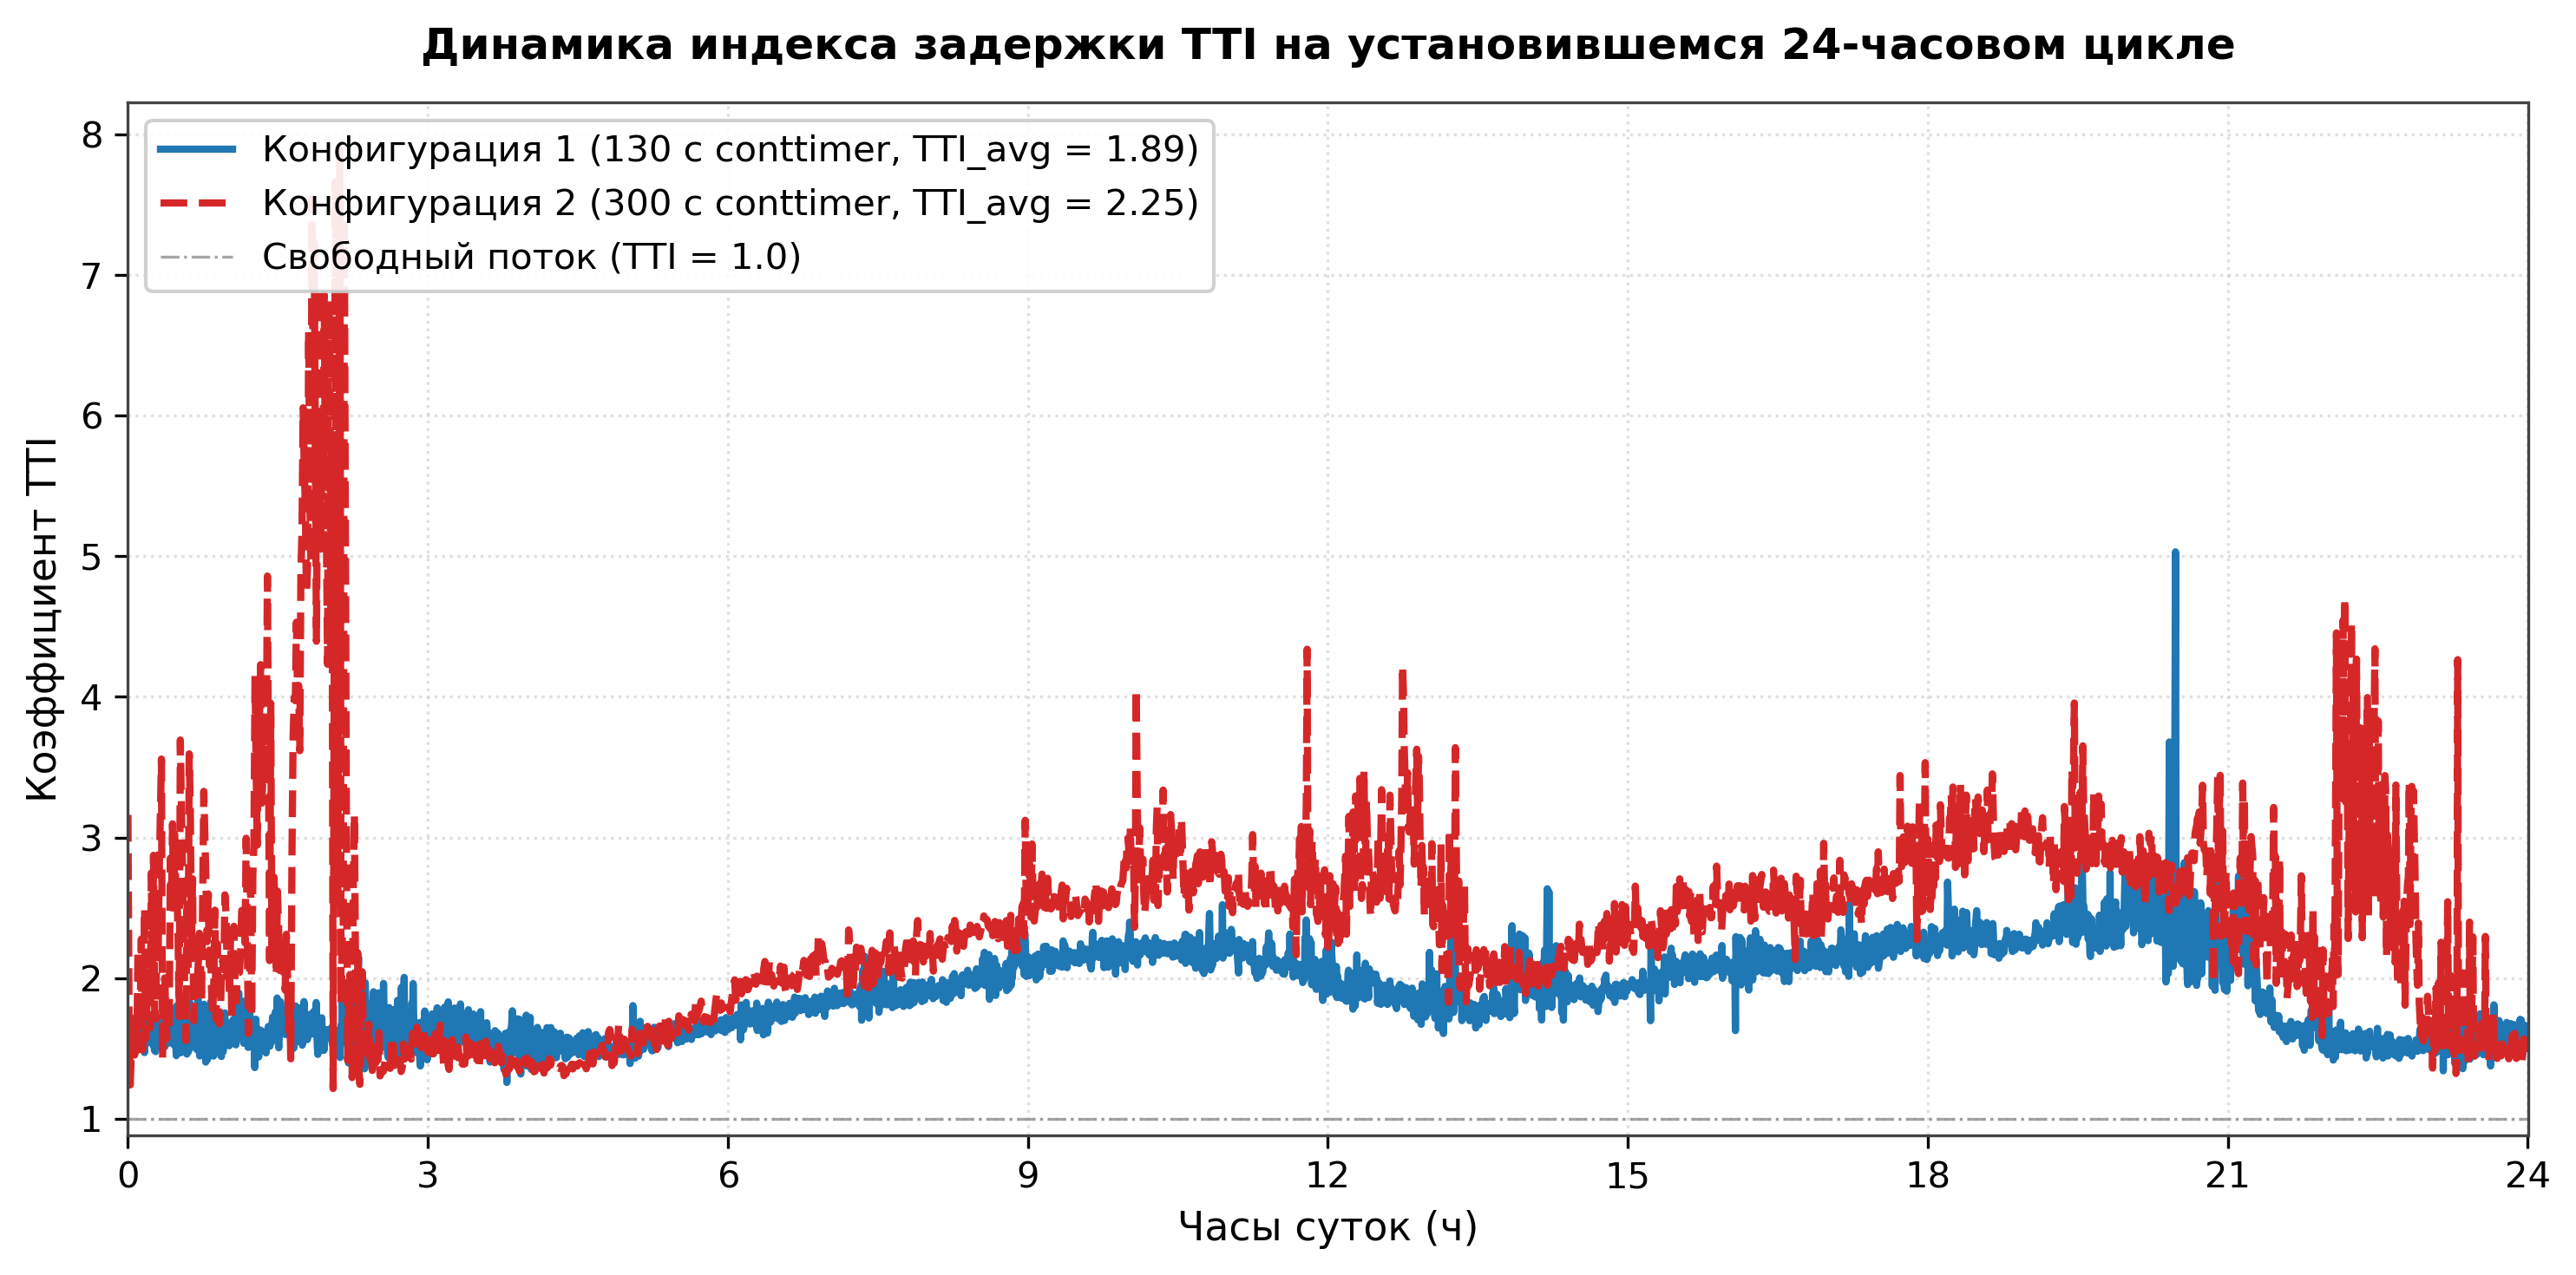
\includegraphics[width=0.95\textwidth]{assets/images/fig_tti_24h.png}
\caption{Динамика индекса задержки TTI на установившемся 24-часовом суточном цикле}
\label{fig:tti_24h}
\end{figure}

На рисунке~\ref{fig:queues_24h} приведено сопоставление накопления и рассасывания различных типов очередей заторов (застрявшие агенты со скоростью 0 км/ч, виртуальный буфер SUMO, очереди перестроения MPR и очереди спавна).

\begin{figure}[h!]
\centering
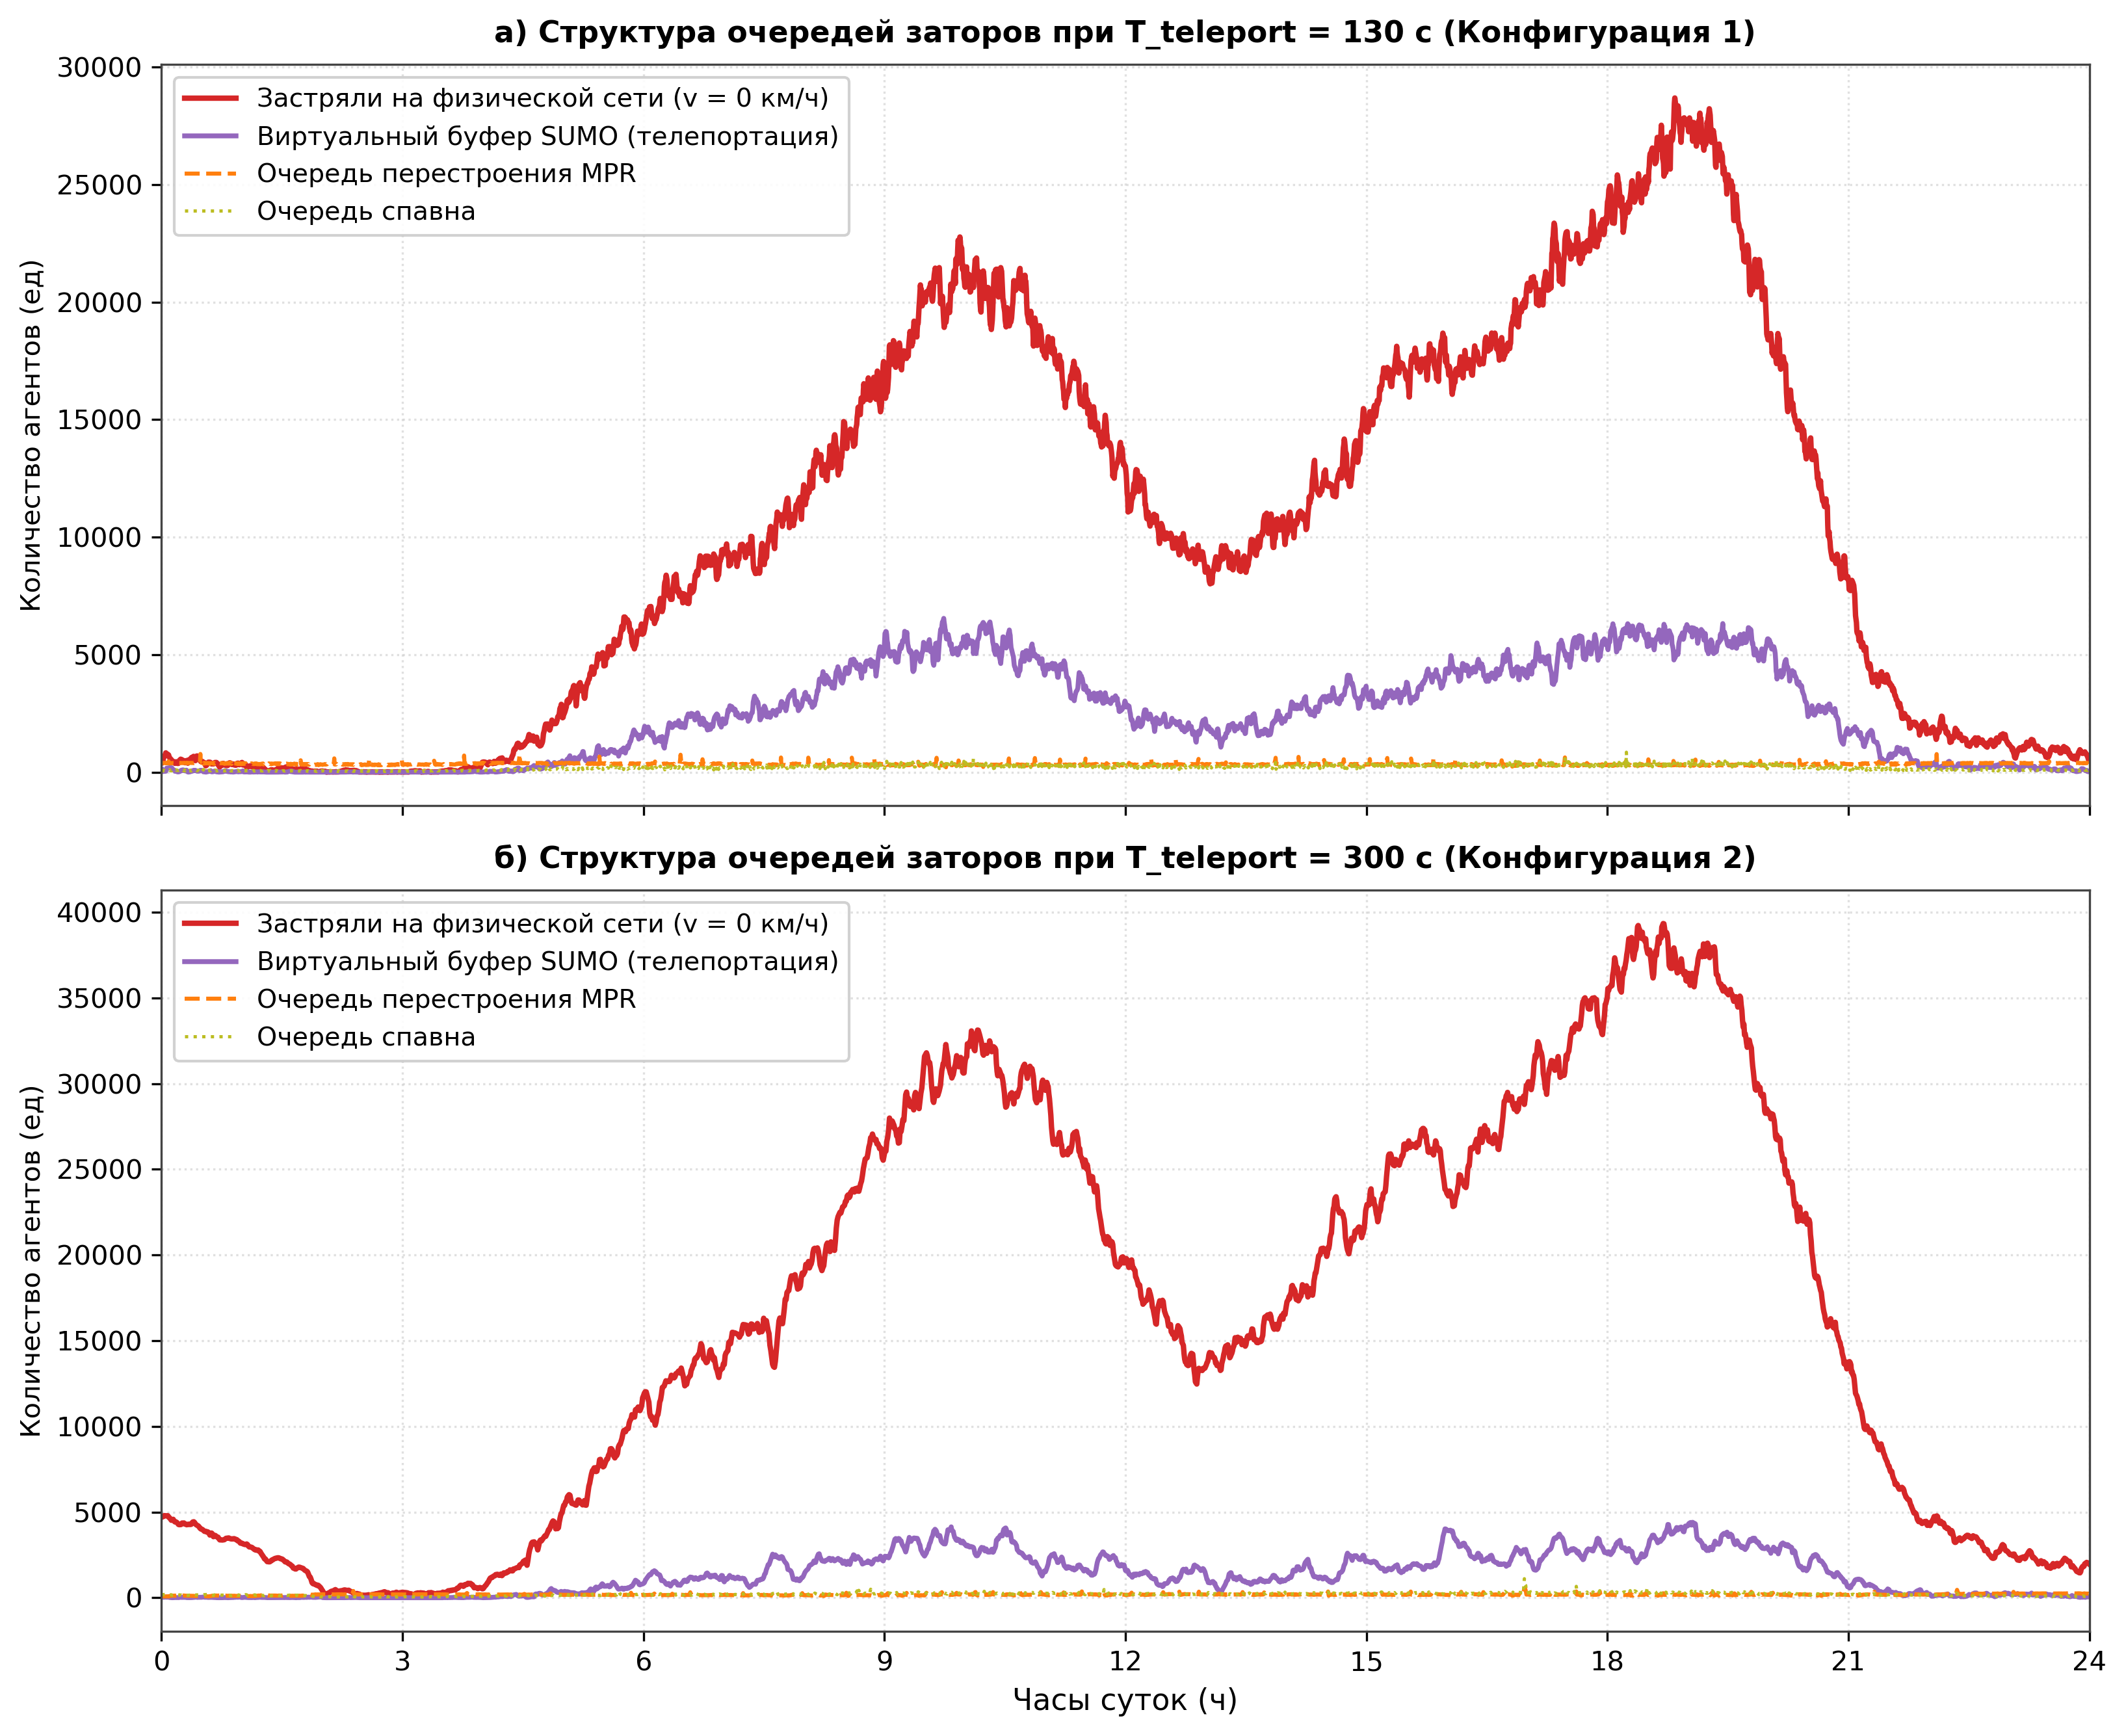
\includegraphics[width=0.95\textwidth]{assets/images/fig_queues_24h.png}
\caption{Динамика накопления и рассасывания очередей заторов на установившемся 24-часовом цикле: а) при $T_{\text{teleport}} = 130$ с; б) при $T_{\text{teleport}} = 300$ с}
\label{fig:queues_24h}
\end{figure}

На рисунке~\ref{fig:zones_24h} показано распределение загруженных ребер дорожной сети по типам зон (красные, желтые и черные зоны) для обеих конфигураций.

\begin{figure}[h!]
\centering
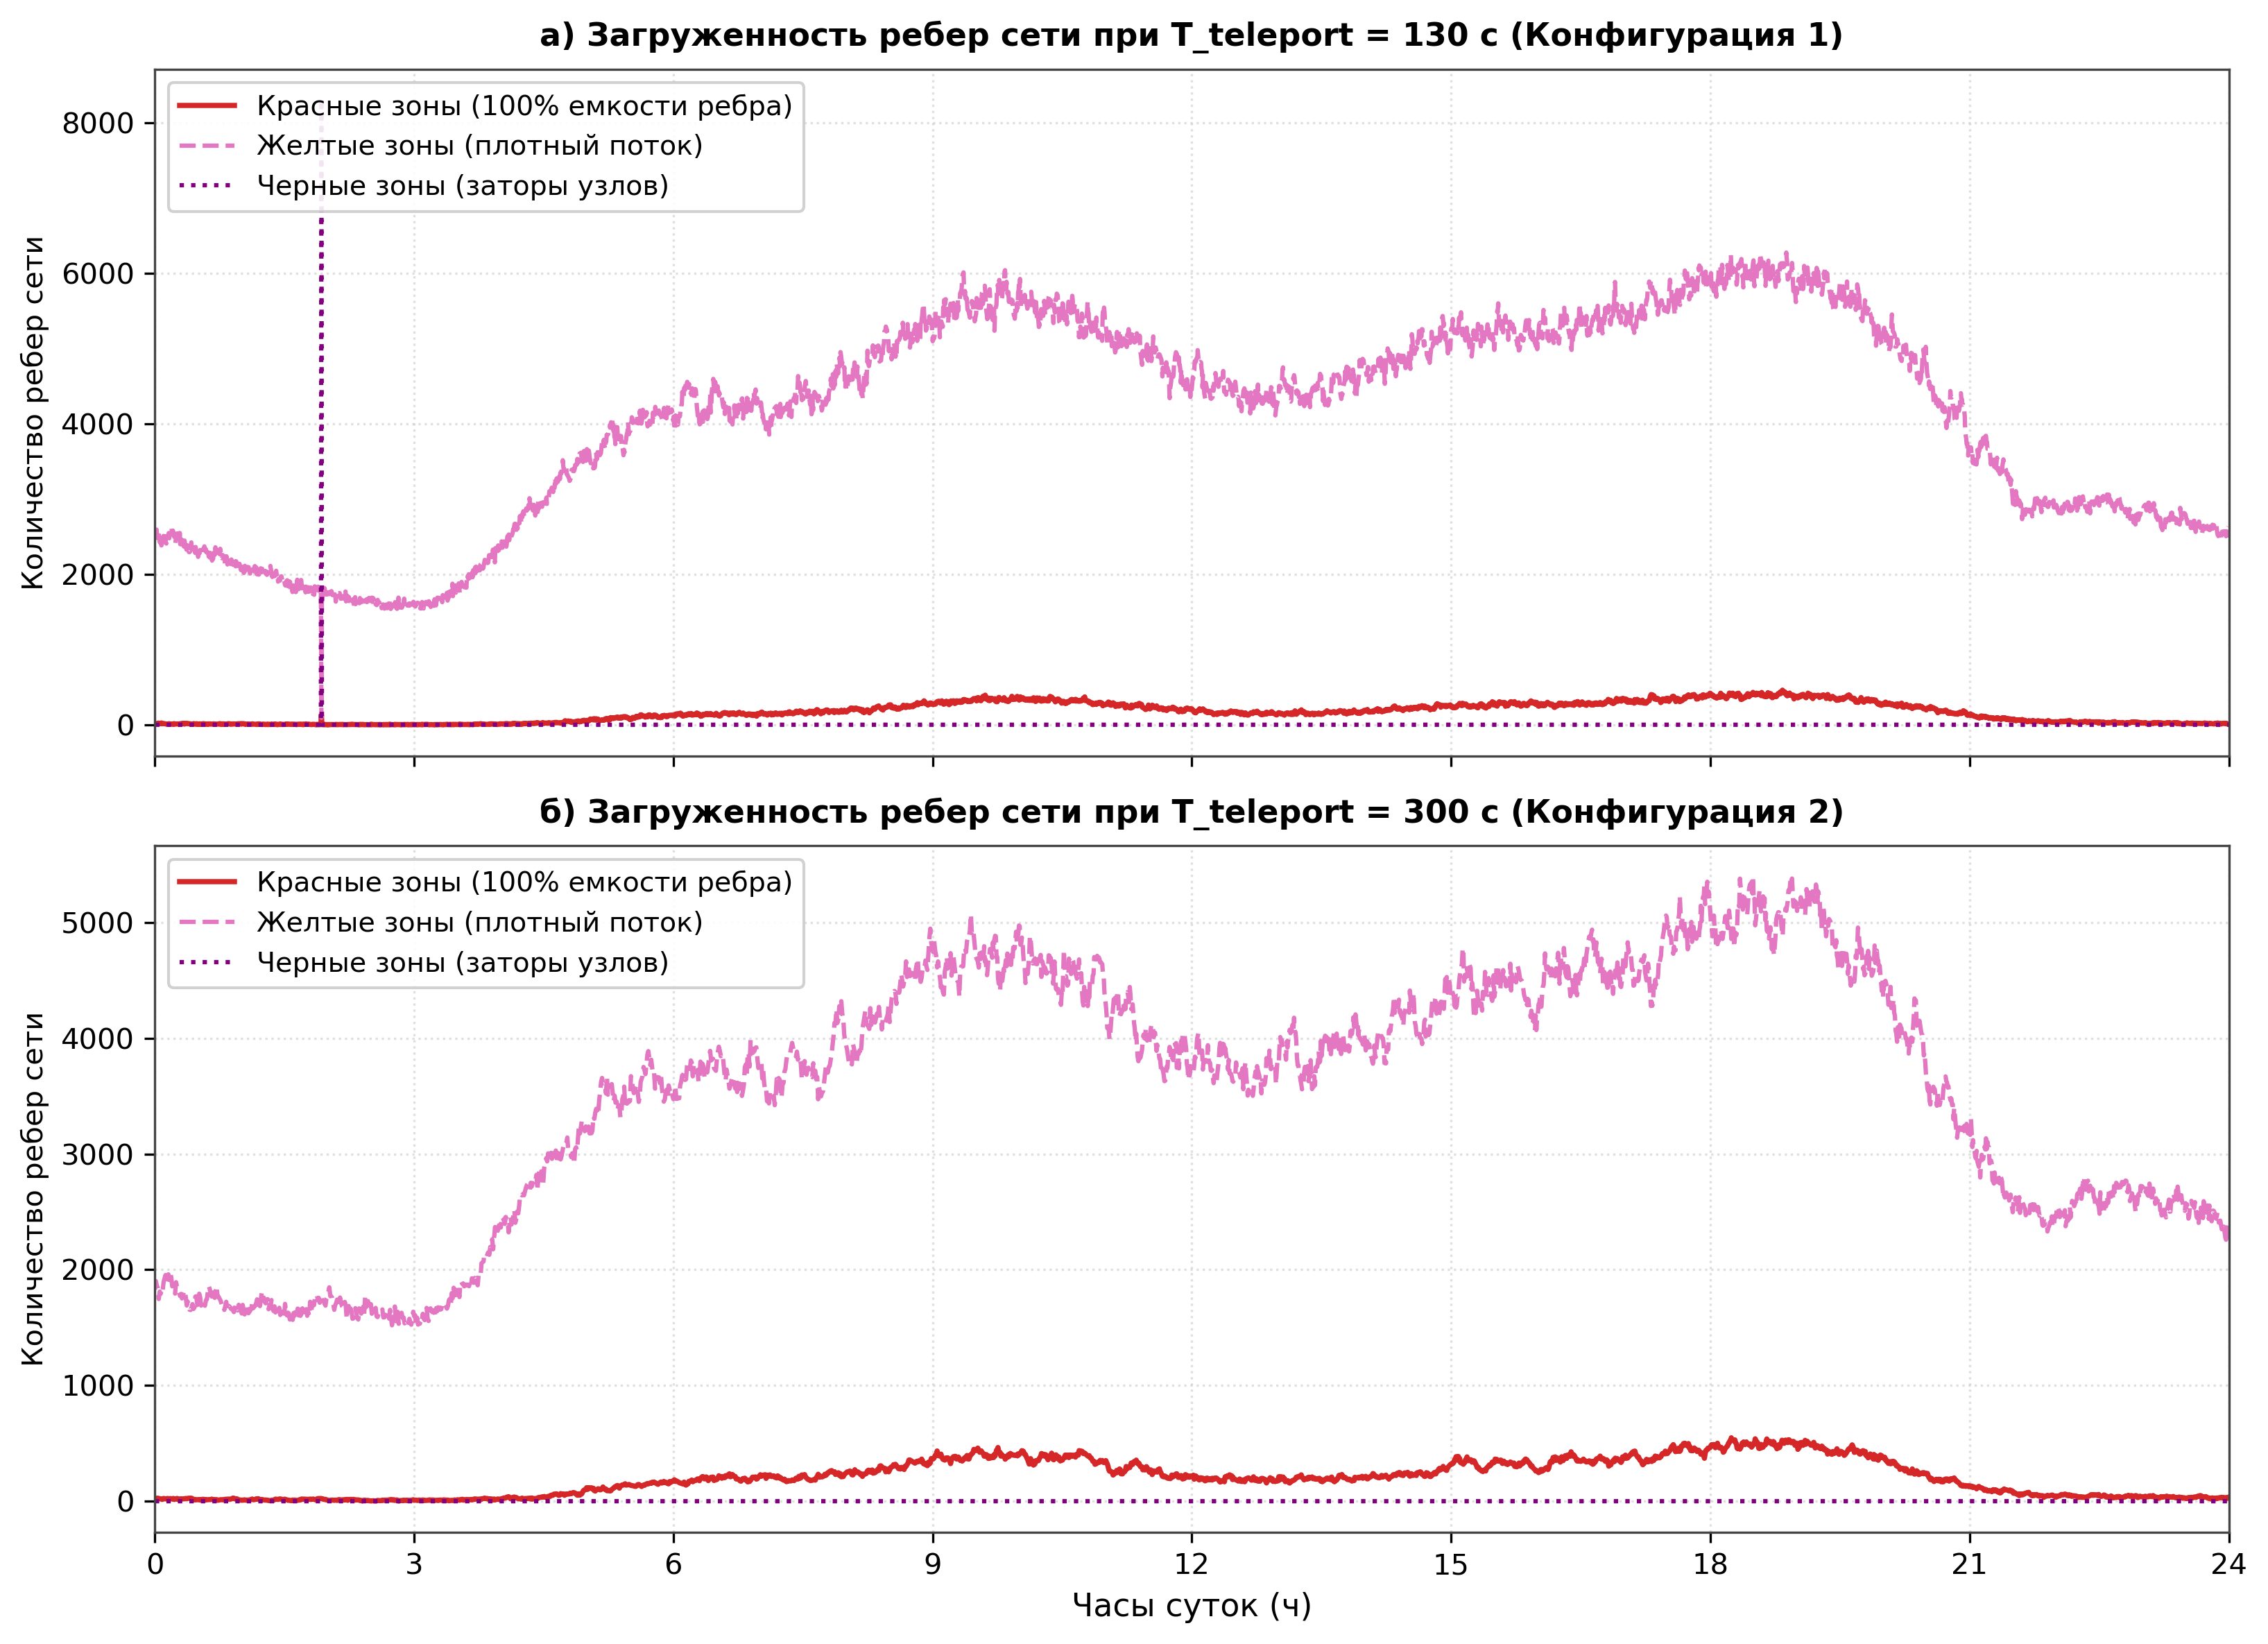
\includegraphics[width=0.95\textwidth]{assets/images/fig_zones_24h.png}
\caption{Распределение плотности ребер сети по уровням заторов (красные, желтые, черные зоны) на установившемся 24-часовом цикле}
\label{fig:zones_24h}
\end{figure}

\section{Анализ показателей TTI, простоя и параметров буфера}
\label{sec:metrics_analysis}

Сравнительный анализ на установившемся 24-часовом цикле показал следующие закономерности:
\begin{enumerate}
    \item При пороговом интервале телепортации $T_{\text{teleport}} = 300$ с накопление застрявших автомобилей со скоростью 0 км/ч достигает пика более $40\,000$ автомобилей в вечерний час пик ($18:00$), что вызывает скачки TTI до уровня $7.89$. При этом виртуальный буфер SUMO не успевает своевременно разгружать короткие ребра.
    \item Уменьшение порога до $T_{\text{teleport}} = 130$ с активизирует своевременную буферизацию агентов в виртуальный слой, снижая количество застрявших на физической сети машин почти в 2 раза (пик снижается до $28\,000$ машин). Индекс TTI в утренний и вечерний часы пик стабилизируется в диапазоне $1.8 \dots 2.2$.
    \item Анализ выборок агентов подтвердил абсолютную целостность данных (\emph{LimboPhantomCount} $= 0$), что указывает на отсутствие потерь автомобилей при циклических операциях перехода в буфер SUMO и обратного спавна.
\end{enumerate}
